\section{Finding Architectural Smell-Inducing Issues}
\label{s:approach}

\begin{figure}
    \centering
    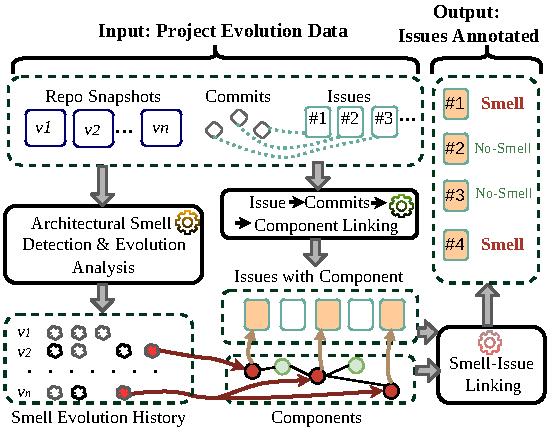
\includegraphics[width=.999\columnwidth,trim=0 0 0 0,clip]{picture/app/approach.pdf}
    \caption{\Acl{ASI} issue identification process}
    \label{fig:dataset-prep}
\end{figure}
This part aims to link architectural smells to their inducing issues. 
We define \ac{ASI} issues as those for which closing them is related to introducing new architectural smells or adding new architectural components to existing smells.
However, due to the nature of issues, they exist in a different domain than architectural smells.
To connect them, we identify and use changes that induce architectural smells.
Specifically, we use four architecture-based static analysis steps:
\textbf{smell detection}, \textbf{smell evolution analysis}, \textbf{issue-component linking}, and \textbf{smell-to-issue linking}.
%HL: Arch recovery can be seen embedded into smell detection (at least in arcan.) then we can skip discussing about multiple recovery approaches
% Given source code repositories across different versions, the architecture recovery step will reconstruct their architecture models.
\autoref{fig:dataset-prep} provides an overview of the process.
Given project repositories across different versions, smell detection will identify architectural smells and annotate each smell's affected components (smelly components).
After that, the results of smell evolution are changes in smells across versions.
After linked to components, issues that affect the smelly components will be annotated as \ac{ASI} issues.

\subsection{Smell Detection}
\label{ss-sec-smellDetec}
This step aims to obtain the evolved \ac{AS} and their affected files throughout the project's evolution.
Based on the affected files, we can link the issues whose resolution was involved.

\paragraph{Version graph and evolution paths}
Release histories of complex systems often involve branching and merging.
% The high-level idea is to  divide and conquer the problem by first decompose complex history into a set of single steps from one version to the next version, then analyzing each single step, finally aggregating results. \todo{simplify}
We therefore model the evolution of a project $P$ as a directed version graph $ G_{Ver} = (V, E)$.
$V$ is the set of versions (releases or commit tags). Each version $v \in V$ is associated with a repository snapshot $Repo(v)$.
$E \subseteq V \times V$ is the set of directed edges, where $(v_i,v_{i+1})$ in $E$ denotes that $v_{i+1}$ directly succeeds $v_i$ (consecutive releases or parent-child in the commit graph).
We can analyze decay step by step along an \emph{evolution path}: $EvoPath = (v_1, v_2, \dots, v_\ell )$.
Such a path can represent the main branch or a release line (e.g., branch 1.x vs.\ 2.x);
if a system contains multiple branches, different paths are analyzed separately.


\paragraph{Smell detection interface}
\label{para:smell-interface}
This module is designed to be tool-agnostic and flexible:
Any architectural smell detection tool can be plugged in, as long as it satisfies the input/output specification defined in \autoref{eq:smell-interface}.

For each version $v$ along an evolution path, we apply an architectural smell detection tool to the snapshot $\mathit{Repo}(v)$.
The tool returns a set of smell instances:
\begin{equation}
    S^v = \{ s_1^v, s_2^v, \dots, s_{k_v}^v \}.
    \label{eq:smell-interface}
\end{equation}
Each smell instance $s \in S^v$ is characterized by:
\begin{enumerate*}[label=(\roman*)]
    \item a smell type $\mathit{type}(s)$ (e.g., dependency cycle, link overload) and
    \item a non-empty set of components $\mathit{Comp}(s)$ in the architecture of version $v$ that participate in the smell.
\end{enumerate*}
This specification aligns with popular architectural smell-detection tools such as \ARCADE~\cite{schmittlaser_ARCADEExtensible_2020} and \Arcan~\cite{sas_ArchitecturalTechnical_2023}.

\subsection{Smell Evolution Analysis}
After applying architectural smell detection to all versions in an evolution path, each version $v$ is annotated with a smell set $S^v$, and, for each smell $s \in S^v$, the corresponding component set $\mathit{Comp}(s)$.
The next step is to analyze how smells evolve between consecutive versions.

\paragraph{Matching smells across versions}
The smell-matching process follows the workflow of the smell evolution tool AStracker~\cite{sas_2022_evolution}.
Consider two consecutive versions $v_1$ and $v_2$ with smell sets $S^{v_1}$ and $S^{v_2}$.
% Smell changes involve adding or removing affected components. %\footnote{Creation and disappearance of smells can be viewed as adding components to an empty set or removing all components to produce an empty set.}
We first group smells by type and compare only smells of the same type (e.g., comparing all dependency-cycle smells with each other, all Hub-like smells with each other).
Within one type, we align individual smell instances based on the overlap of their component sets.

Given two smells $s^1 \in S^{v_1}$ and $s^2 \in S^{v_2}$ of the same type, we measure their similarity using the Jaccard index over their component sets $\mathit{Comp}(\cdot)$:
\begin{equation}
    \label{eq:jac}
    J(s^1, s^2) =
    \frac{\left| \mathit{Comp}(s^1) \cap \mathit{Comp}(s^2) \right|}
    {\left| \mathit{Comp}(s^1) \cup \mathit{Comp}(s^2) \right|}
\end{equation}
Two smells are considered a match if
\begin{enumerate*}[label=(\roman*)]
    \item they have the same type and
    \item their Jaccard similarity is at least above a threshold $\theta$ (hyperparameter).
\end{enumerate*}

\paragraph{Evolution categories}
Using the matching result from an edge $(v_1, v_2)$, we classify smell changes involved in this step into four categories:
\begin{itemize}[leftmargin=*]
    \item \textbf{Remaining}: matched pairs $(s^1, s^2)$ where $\mathit{Comp}(s^1)$ and $\mathit{Comp}(s^2)$ are identical (same components).
    \item \textbf{Modified}: matched pairs $(s^1, s^2)$ where $\mathit{Comp}(s^1)$ and $\mathit{Comp}(s^2)$ differ (some components were added or removed from the smell, but some are not changed).
    \item \textbf{Removed}: smells in $S^{v_1}$ that have no match in $S^{v_2}$.
    \item \textbf{Added}: smells in $S^{v_2}$ that have no match in $S^{v_1}$.
\end{itemize}

Since we aim to identify issues that induce smells, we target at where smells \textbf{deteriorate}: added smells or modified smells with added component(s). 
We define these two cases as \gs, which will be used for linking.
% Since we aim to identify \gs, we only consider added smells and modified smells with added components.

% \subsection{}
% The procedure consists of two phases:
% (1) establishing \emph{component--issue linking} that maps issues to the components they structurally modify, and
% (2) \emph{evolution matching} that maps \gs to issues based on component overlap.

\subsection{Issue-Component Linking}
\label{subsec:issue-linking}
The remaining steps aim for linking \gs back to the implementation issues whose resolution contributed to their growth.
Our key idea is to use components as the bridge between issues and smells.
This step answers the question: for an issue, which component(s) did its implementation affect?
Issue implementations are realized as commit(s) at the file level, whereas architectural smells are defined at the component level.
We therefore first identify structurally relevant commits and then lift file-level changes to components.

Not all file changes are architecturally relevant.
Developers frequently modify code that does not affect structural dependencies.
To reduce noise, we restrict ourselves to commits that modify structural relations, such as \texttt{import} or \texttt{\#include} statements.
For an issue $i$, let $\mathit{Cmt}(i)$ denote the set of linked commits that modify structural dependencies.

From each commit $c \in \mathit{Cmt}(i)$, we extract the set of files whose dependencies changed; let $\mathit{F}(c)$ denote this set.
The union over all such commits is the structurally affected files of issue $i$:
$\mathit{F}(i) = \{ f \mid c \in \mathit{Cmt}(i),\, f \in \mathit{F}(c) \}$

Based on component-file mapping $\mathit{F}(c)$ (the set of files belonging to component $c$), we derive the affected components:
\begin{equation}
    \label{eq:comptrace}
    \mathit{CompTrace}(i) = \{ c \mid \mathit{F}(c) \cap \mathit{F}(i) \neq \emptyset \}
\end{equation}
Thus, for each issue $i$, we obtain the set of components whose structural dependencies were touched.



\subsection{Growing Smells to Issue Linking}
This step links \gs to issues via components.
Given a \gs $s$ with a step $(v_i, v_{i+1})$, we determine which components were changed in this smell.
We distinguish by evolution category:

\begin{itemize}[leftmargin=*]
    \item For \textbf{modified} smells, the relevant components are the components newly added to the smell, 
    % i.e.\ components that were not part of the smell in $v_i$ but appear in $v_{i+1}$.
    \item For \textbf{added} smells, the relevant components are all components in the new smell instance in $v_{i+1}$.
\end{itemize}
We denote this set by $\mathit{RelComp}(s)$.

For an issue $i$, we quantify how strongly it is involved in the evolution of $s$ by the ratio of relevant components that were touched by the issue (as given by \autoref{eq:comptrace}):
\begin{equation}
    \mathit{overlap}(s, i) =
    \frac{ \left| \mathit{RelComp}(s) \cap \mathit{CompTrace}(i) \right| }
    { \left| \mathit{RelComp}(s) \right| }
    \label{eq-overlap-si}
\end{equation}
An $\mathit{overlap}$ of $1.0$ means that all relevant components of the smell were modified in the issue; any positive value indicates partial component-level involvement in the issue.

We link an issue $i$ to an evolved smell $s$ on edge $(v_i, v_{i+1})$ if both of the following hold:
\begin{enumerate}[leftmargin=*]
    \item The commits implementing $i$ fall within the time interval corresponding to the evolution from $v_i$ to $v_{i+1}$, and
    \item $\mathit{overlap}(s, i) > \gamma$, where $\gamma$ is a threshold hyperparameter.
\end{enumerate}


The final output is a set of annotated \ac{ASI} issues:
\begin{align}
    \textit{ASI-Issues} =
    \{ (i, s, \mathit{overlap}(s,i)) \mid\;
     & s \text{ is a growing smell,} \nonumber \\
     & i \text{ is linked to } s \}.
\end{align}

Each tuple $(i, s, \mathit{overlap}(s,i))$ captures how strongly issue $i$ contributed to the growth of smell $s$.
This enables downstream analyses such as training classifiers to predict \acl{ASI} issues from issue texts
and studying characteristics of issues that tend to cause architectural decay.











\section{\approach: Predicting Smell-Inducing Issues}

Given the annotated set of architecturally smelly issues, we define the following prediction task:
determining whether an issue will induce an architectural smell \emph{during the design stage}, before any implementation occurs.
This task relies solely on information available at design time: the issue title, description, and optionally early-stage discussions.

Our prediction pipeline extracts and leverages semantic signals from these textual artifacts.
We investigate three complementary categories of predictive approaches:
\begin{enumerate*}[label=(\roman*)]
    \item encoding-based vector classification models,
    \item prompting decoder-based \acp{LLM}, and
    \item fine-tuning encoder-based \acp{LLM}.
\end{enumerate*}
Each category offers distinct advantages.
Encoding-based models are scalable and inexpensive to deploy, prompting-based approaches leverage the rich prior knowledge of pre-trained \acp{LLM}, and fine-tuned \acp{LLM} can exploit domain-specific patterns by adapting model parameters to the task.

\subsection{Encoding-Based Classification}
For encoding-based classification, we map each issue to a fixed-dimensional vector with an \textbf{encoder} and apply lightweight supervised \textbf{classifiers}.
These classifiers offer low cost, high interpretability, and extensibility.

\paragraph{Encoders}
Encoders transform texts into vectors suitable for classification.
To cover main categories of text representations, we use the following encoders 

\textbf{TF--IDF} is a distribution-based vector representation for capturing token importance across all project texts.
It calculates token frequency and then normalized by document frequency.
As a statistical model, it is cheap to compute and requires no pre-training to obtain vectors.

Embeddings using small language models (SLMs), i.e., \textbf{\acf{SBERT} embeddings}, fine-tuned on text similarity tasks distinguish semantic meaning and produce dense contextual embeddings.
For issues exceeding the 512 token context window of \ac{SBERT}, we split texts into chunks, encode each independently, and aggregate chunk vectors using pooling (e.g., average, max). 

Lastly, we use \textbf{\ac{LLM}-based embeddings} (OpenAI's text-embedding-3-small) with an 8k-token context window (16x larger than \ac{SBERT}).

\paragraph{Classifier}
After issue-level vector construction, we apply vector-based classification models.
We consider common classifiers such as \textbf{\ac{ffNN}}, \textbf{\ac{NB}}, \textbf{\ac{LR}}, \textbf{\ac{RF}}, \textbf{\ac{SVM}}, \textbf{\ac{XGB}} models, and \textbf{\ac{kNN}}.
Their low inference cost and ease of tuning make these models suitable for large-scale deployment scenarios.

\subsection{Fine-tuning Language Models}
\label{sec:roberta}
To evaluate the benefits of end-to-end learning, we fine-tune a RoBERTa model for binary classification of \ac{ASI} versus non–\ac{ASI} issues.
Fine-tuning allows the model to learn project-specific terminology and cues.
As with SentenceBert, issue texts often exceed RoBERTa’s context window (512 tokens).
Therefore, we need a design that ensures complete coverage of long issues, while enabling RoBERTa to analyze localized semantic signals within each chunk.
Thus, we apply \textbf{Issue Chunking Aggregation}, where issues got splitted into chunks, classified separately, and aggregated.
We use the mean of each chunk's result to obtain the result on issue-level.
The impact of the design choices will be evaluated in \ref{RQ2 Performance comparison}.

\subsection{Prompting LLMs}
\label{sec:llm-based}
We complement supervised approaches with prompting \acp{LLM} to measure the intrinsic architectural reasoning capabilities of pretrained models.
%We consider 0-shot prompts and chain-of-thought prompting.
%\paragraph{Zero-shot prompting.}
We provide the \ac{LLM} with the issue text and a task description to classify whether the issue is likely to trigger architectural smell evolution:
\begin{promptR}{Zero-Shot Prompt}{zero}\\
    You are an expert software architect analyzing Gitlab issues.\\
    \{SMELL\_DEFINITIONS\}\\
    Issue:\\
    \{TEXT\}\\
    % Classify as smell or no\_smell based on whether it describes architectural problems.\\
    Classify as smell or no\_smell based on if resolving this issue would cause architectural smells defined above.\\
    Respond ONLY with a JSON object containing: \\
 classification: either smell or no\_smell \\
 reason: a short justification \\
Do not include code fences or extra narration.
\end{promptR}
\noindent For \ARCADE we provide the following smell definition:

\textit{An architectural smell is a design problem indicating violations of fundamental design principles:
    \begin{itemize}[label=--,leftmargin=*]
        \item Big Dependency Cycle (BDC): Circular dependencies between components violating architectural layering
        \item Link Overload (LO): One component has too many dependencies
    \end{itemize}}
% \noindent For \Arcan the definition additionally includes: %\footnote{In \Arcan, link overload smell are named as hub-like smell}:
% \textit{\begin{itemize}[label=--,leftmargin=*]
%         \item Unstable dependencies (UD): A component depends on another component that is less stable than itself
%     \end{itemize}}
For \Arcan, we also define its supporting smells. Its prompt can be found in replication package\cite{replication}.
